\thispagestyle{fancy}
\vspace*{40 pt}
\subsection{Vista geral dos ajustes das impressoras}
\vspace*{\fill}
\begin{figure}[h]
    \centering
    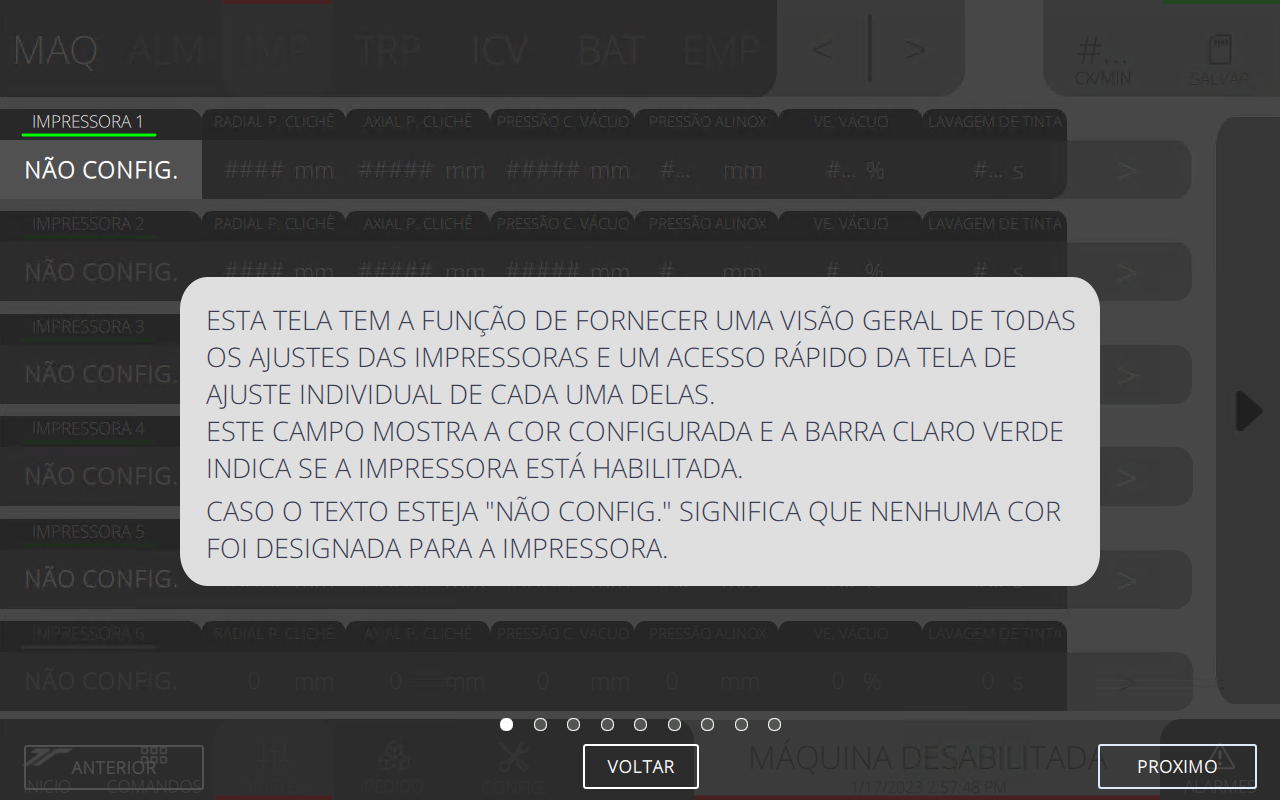
\includegraphics[width=480 px,height=300 px]{src/imagesICV/04-printters/01-printters/settings/1.png}
\end{figure}
\vspace*{\fill}

\newpage
\thispagestyle{fancy}
\vspace*{40 pt}
\subsection{Aproximação do anilox bloqueada}
\vspace*{\fill}
\begin{figure}[h]
    \centering
    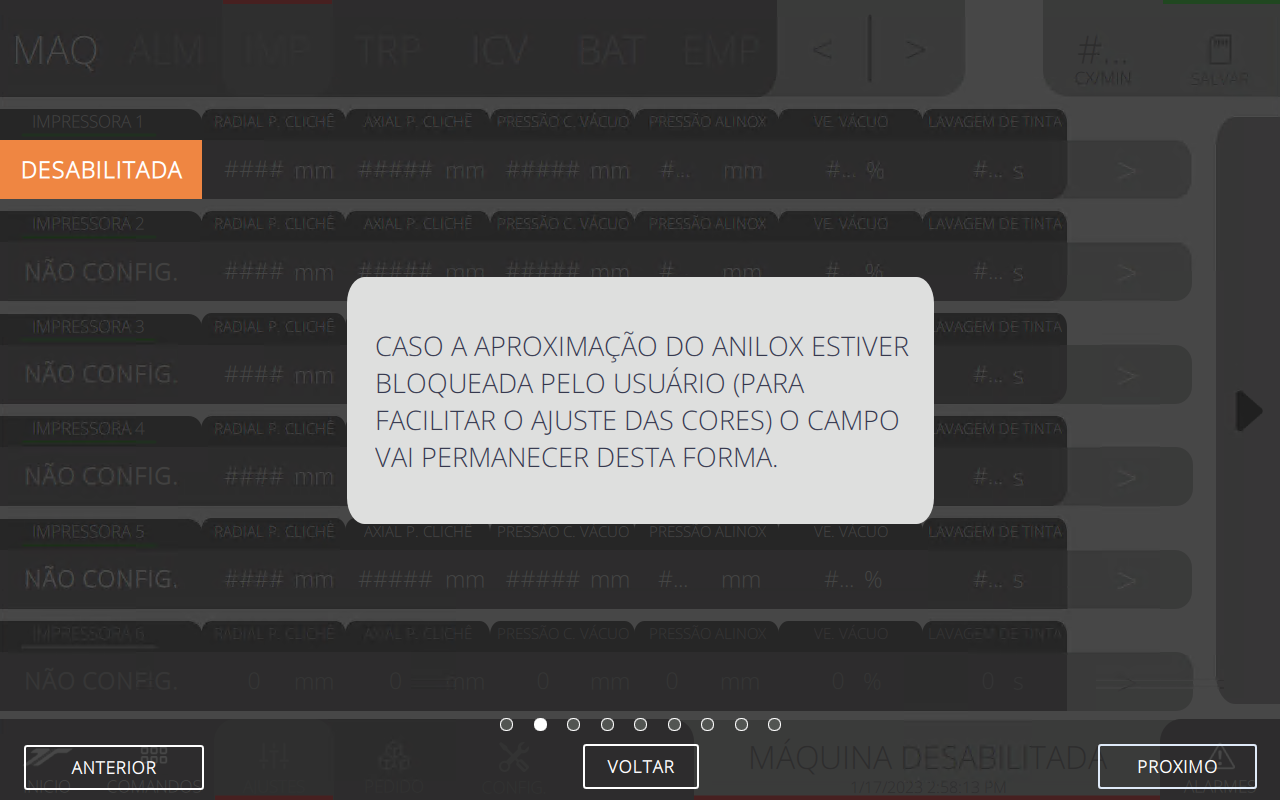
\includegraphics[width=576 px,height=360 px]{src/imagesICV/04-printters/01-printters/settings/2.png}
\end{figure}
\vspace*{\fill}

\newpage
\thispagestyle{fancy}
\vspace*{40 pt}
\subsection{Registro atual}
\vspace*{\fill}
\begin{figure}[h]
    \centering
    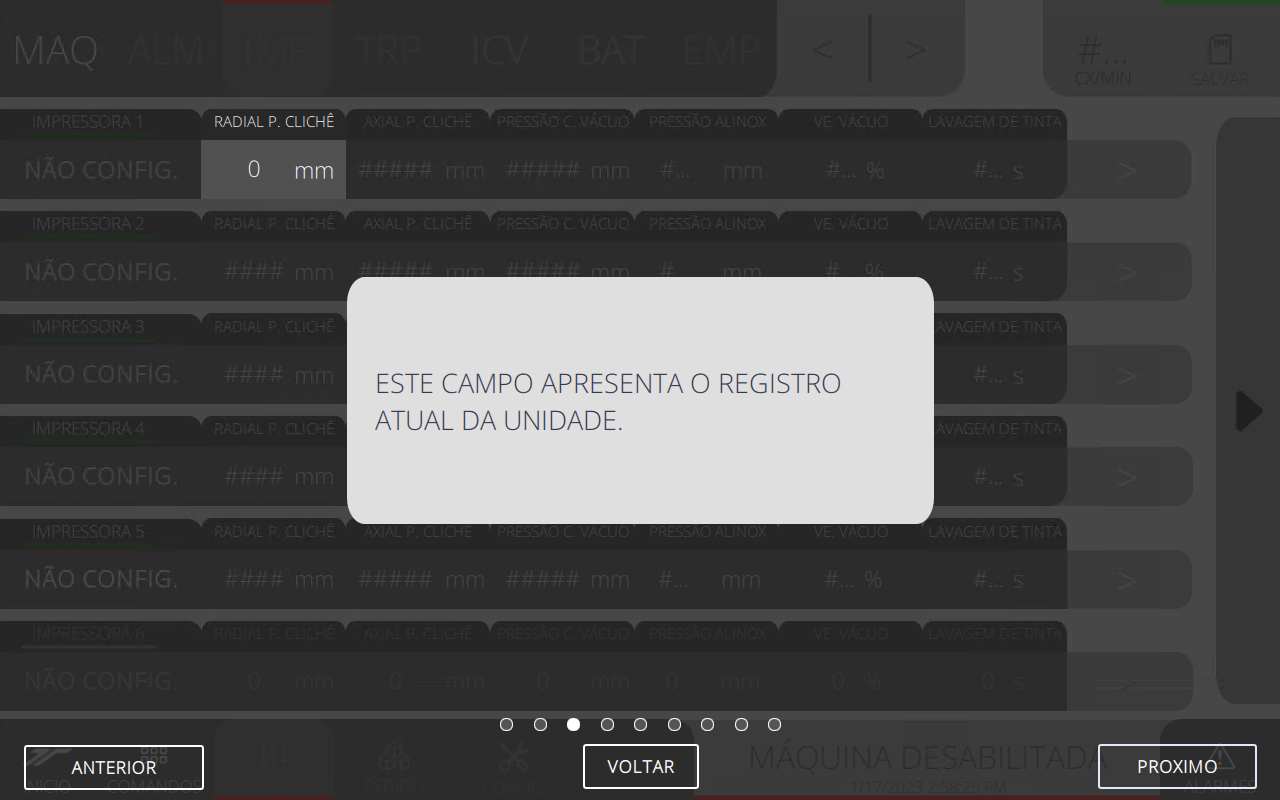
\includegraphics[width=576 px,height=360 px]{src/imagesICV/04-printters/01-printters/settings/3.png}
\end{figure}
\vspace*{\fill}

\newpage
\thispagestyle{fancy}
\vspace*{40 pt}
\subsection{Ajuste axial do Clichê}
\vspace*{\fill}
\begin{figure}[h]
    \centering
    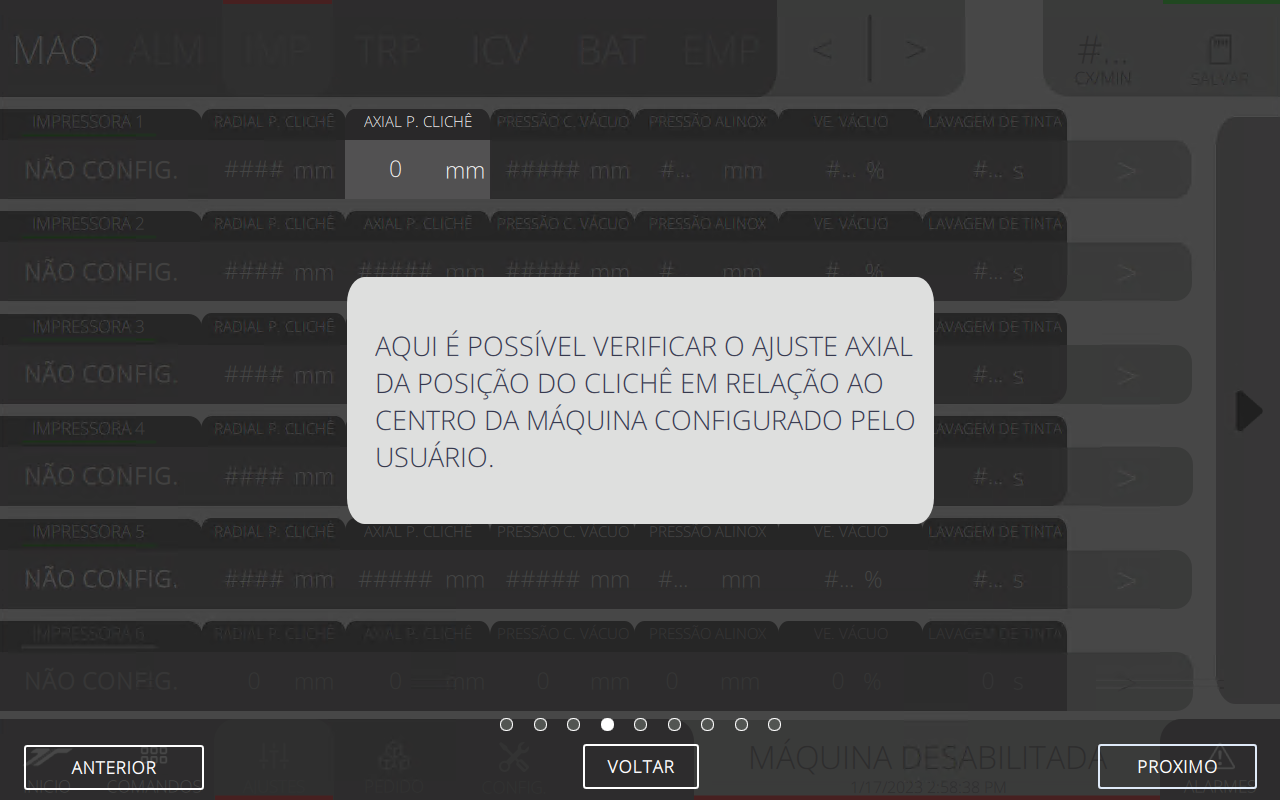
\includegraphics[width=576 px,height=360 px]{src/imagesICV/04-printters/01-printters/settings/4.png}
\end{figure}
\vspace*{\fill}

\newpage
\thispagestyle{fancy}
\vspace*{40 pt}
\subsection{Pressão caixa de vácuo}
\vspace*{\fill}
\begin{figure}[h]
    \centering
    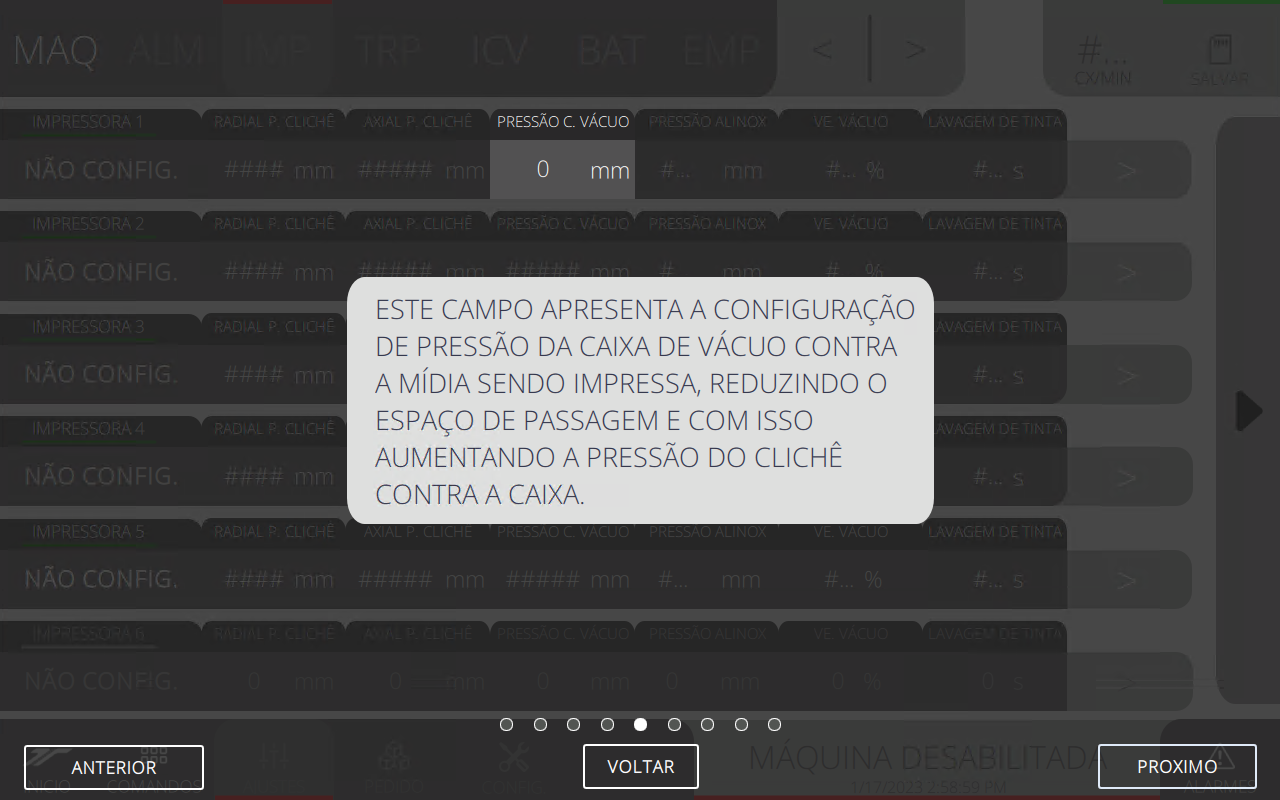
\includegraphics[width=576 px,height=360 px]{src/imagesICV/04-printters/01-printters/settings/5.png}
\end{figure}
\vspace*{\fill}

\newpage
\thispagestyle{fancy}
\vspace*{40 pt}
\subsection{Pressão anilox}
\vspace*{\fill}
\begin{figure}[h]
    \centering
    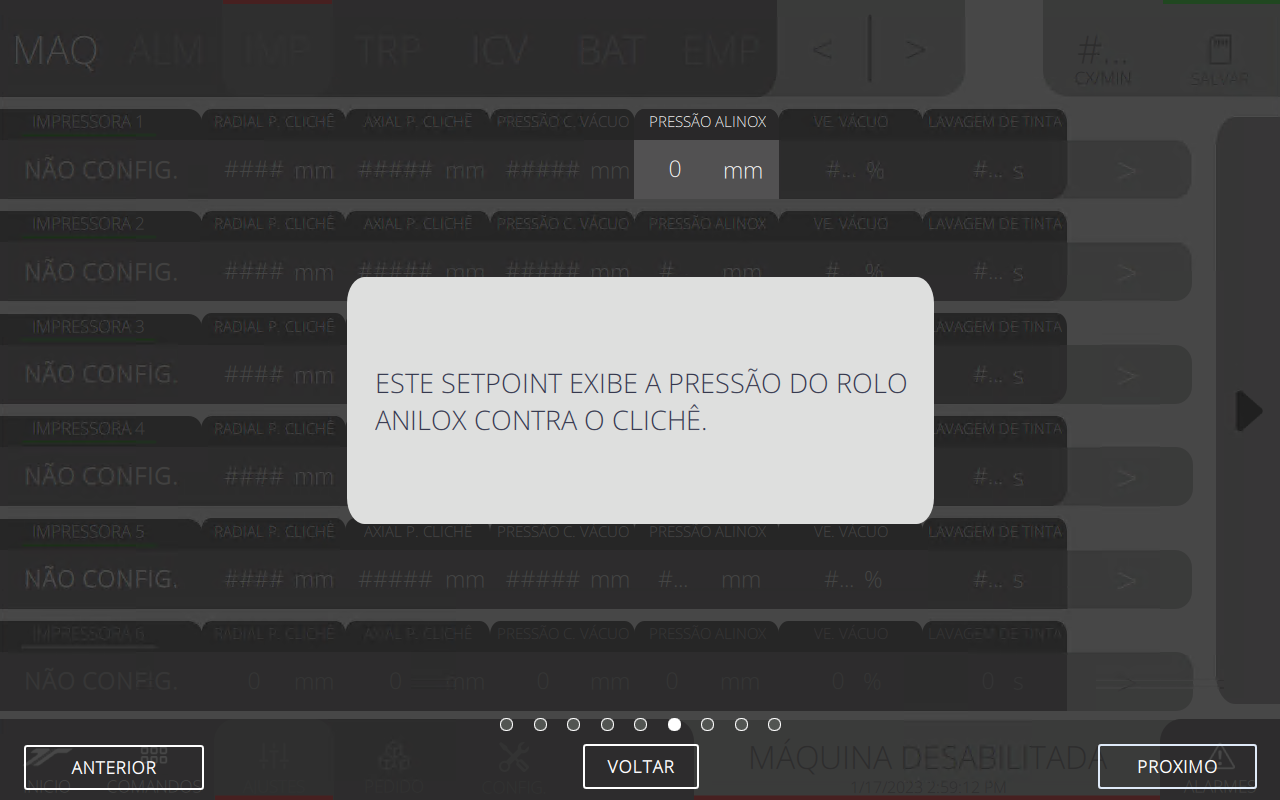
\includegraphics[width=576 px,height=360 px]{src/imagesICV/04-printters/01-printters/settings/6.png}
\end{figure}
\vspace*{\fill}

\newpage
\thispagestyle{fancy}
\vspace*{40 pt}
\subsection{Intensidade do vácuo}
\vspace*{\fill}
\begin{figure}[h]
    \centering
    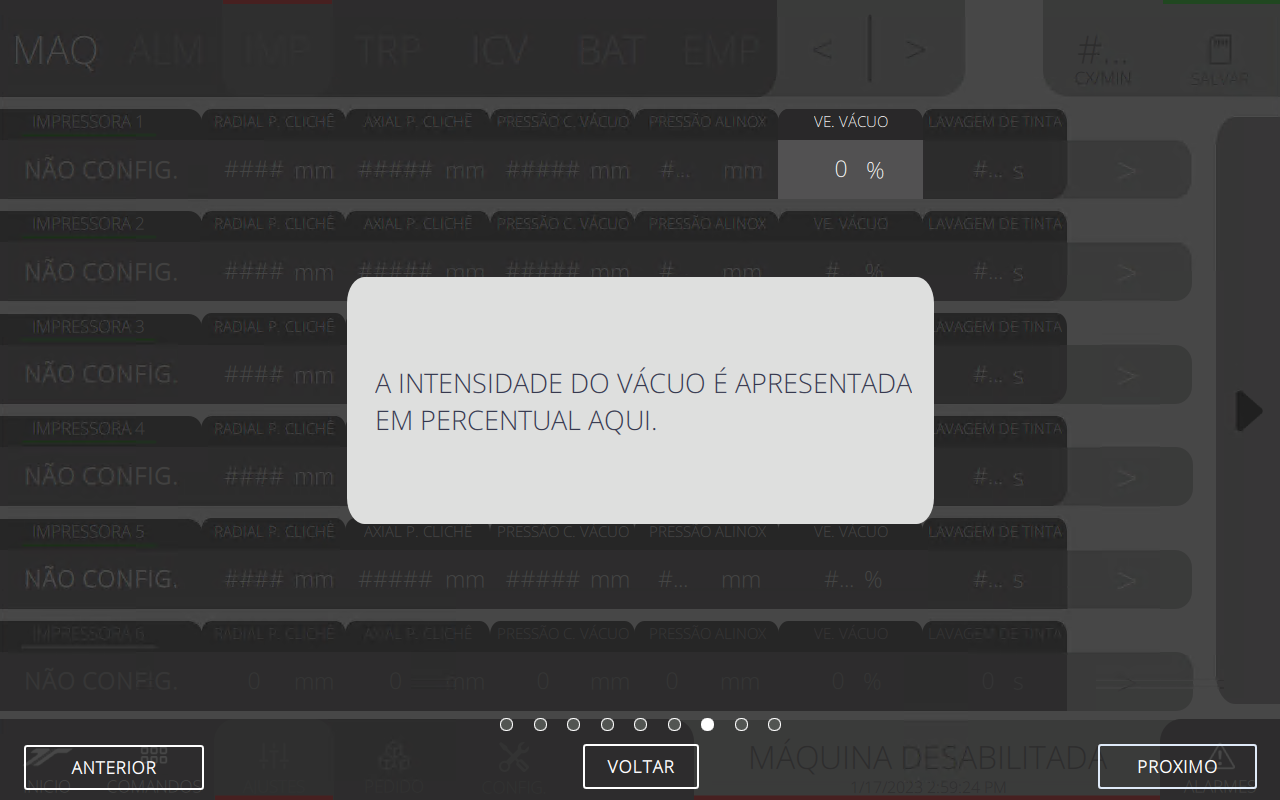
\includegraphics[width=576 px,height=360 px]{src/imagesICV/04-printters/01-printters/settings/7.png}
\end{figure}
\vspace*{\fill}

\newpage
\thispagestyle{fancy}
\vspace*{40 pt}
\subsection{Tempo ativo da lavagem de tinta}
\vspace*{\fill}
\begin{figure}[h]
    \centering
    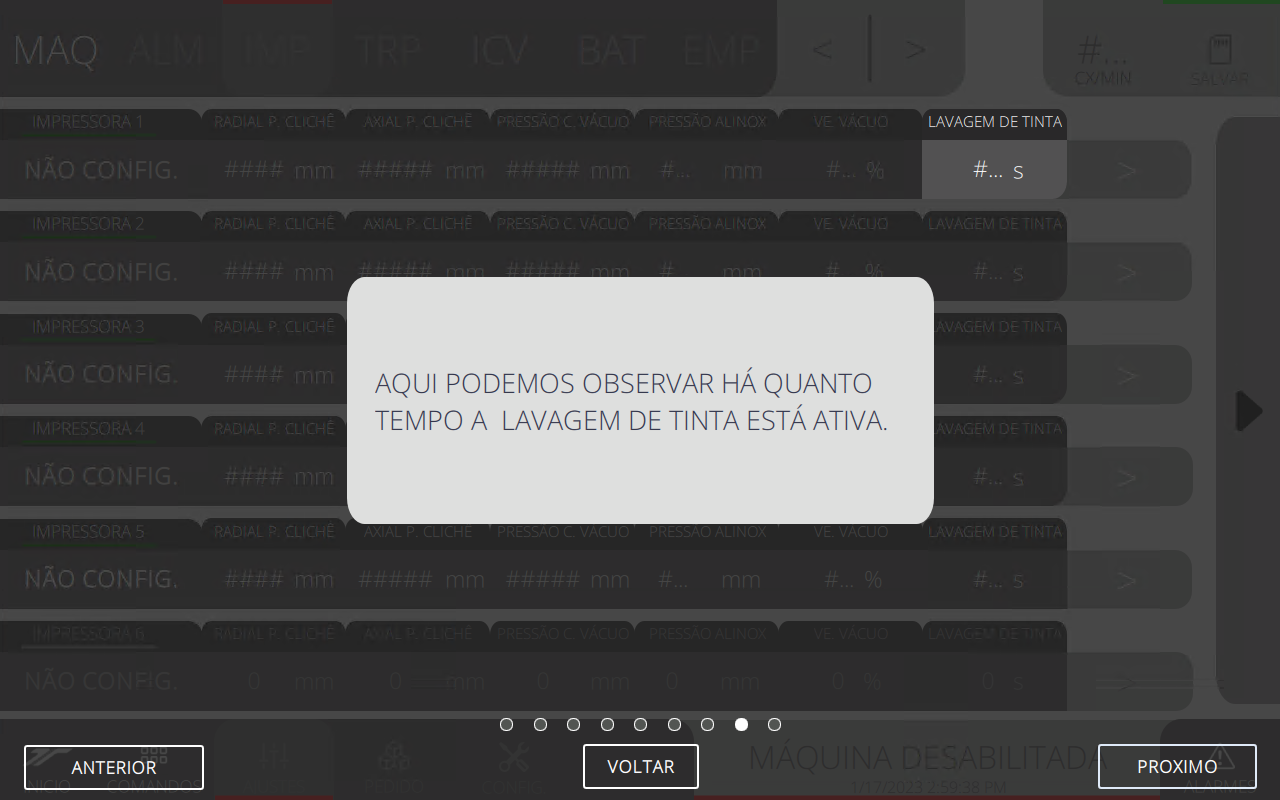
\includegraphics[width=576 px,height=360 px]{src/imagesICV/04-printters/01-printters/settings/8.png}
\end{figure}
\vspace*{\fill}

\newpage
\thispagestyle{fancy}
\vspace*{40 pt}
\subsection{Ajuste individual da unidade}
\vspace*{\fill}
\begin{figure}[h]
    \centering
    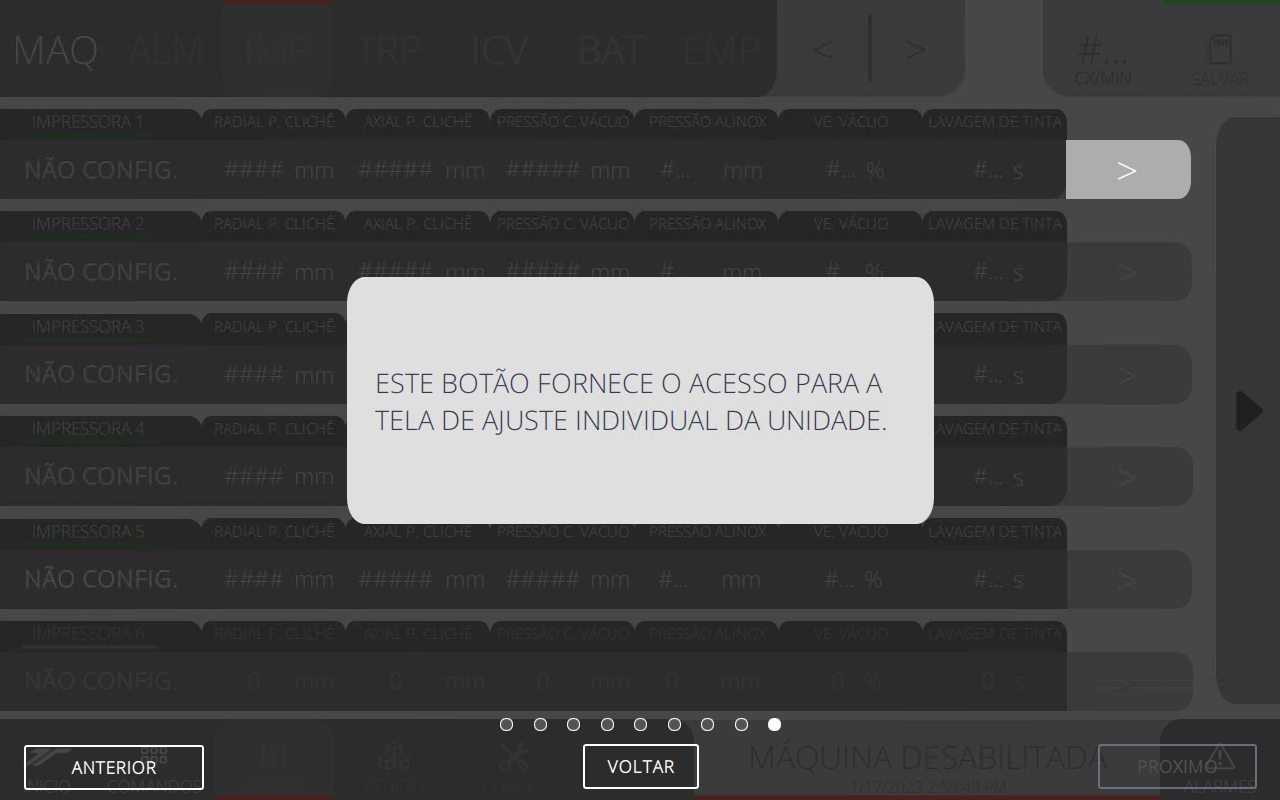
\includegraphics[width=576 px,height=360 px]{src/imagesICV/04-printters/01-printters/settings/9.png}
\end{figure}
\vspace*{\fill}

\newpage
\thispagestyle{fancy}
\vspace*{40 pt}
\subsection{Axial porta clichê}
\vspace*{\fill}
\begin{figure}[h]
    \centering
    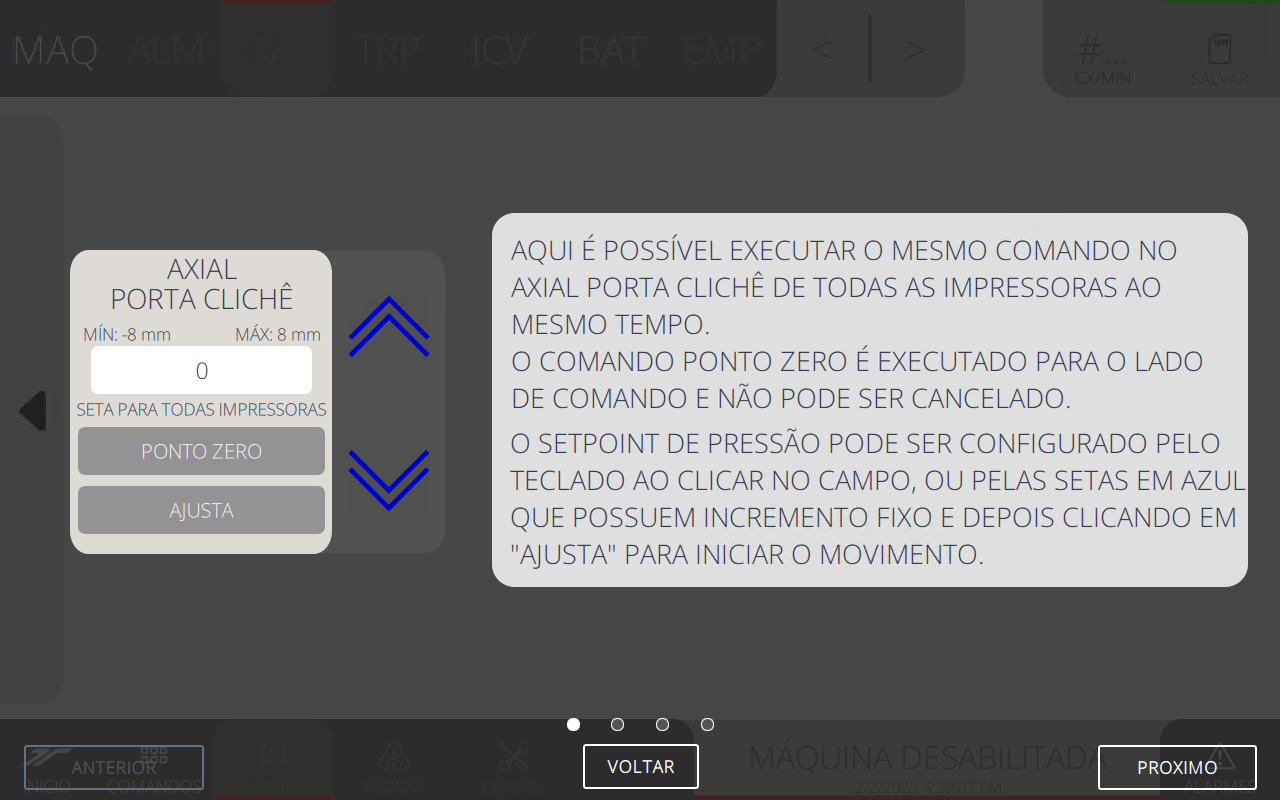
\includegraphics[width=576 px,height=360 px]{src/imagesICV/04-printters/01-printters/settings/10.png}
\end{figure}
\vspace*{\fill}

\newpage
\thispagestyle{fancy}
\vspace*{40 pt}
\subsection{Pressão caixa de vácuo}
\vspace*{\fill}
\begin{figure}[h]
    \centering
    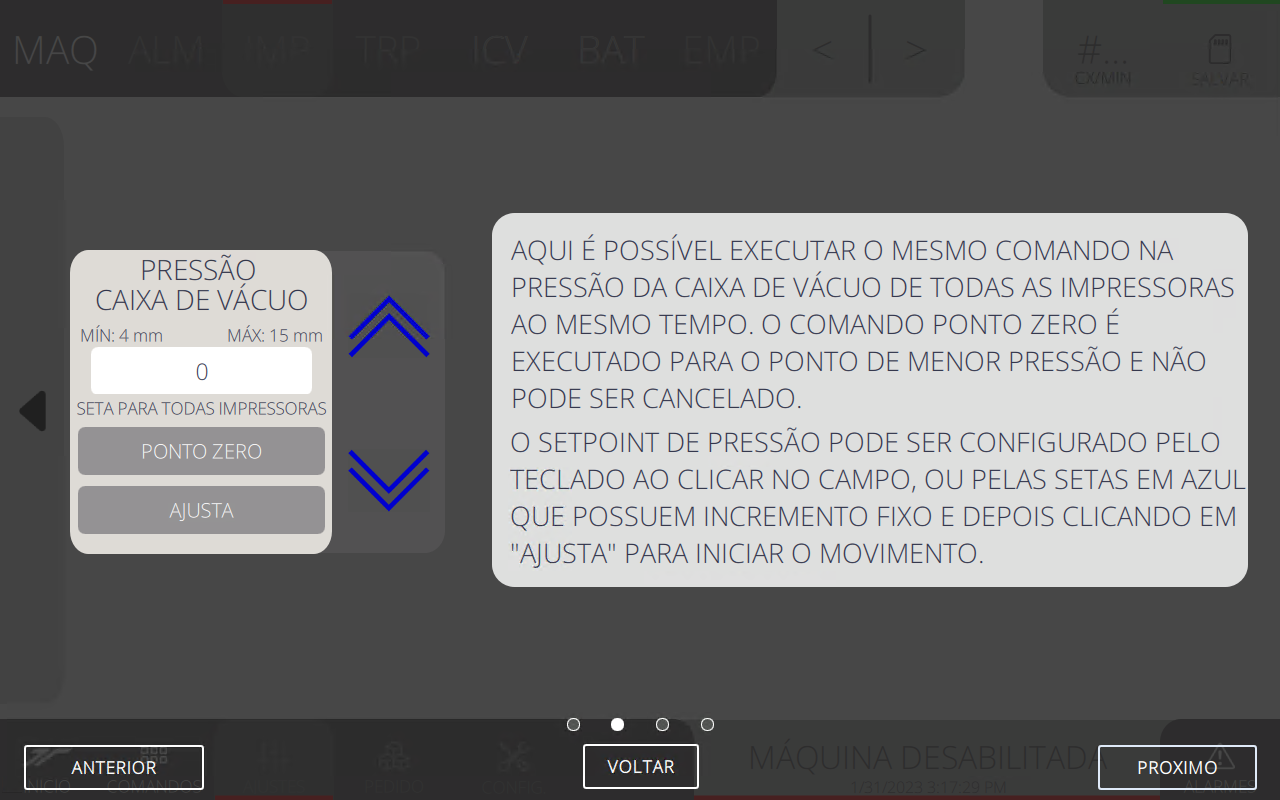
\includegraphics[width=576 px,height=360 px]{src/imagesICV/04-printters/01-printters/settings/11.png}
\end{figure}
\vspace*{\fill}

\newpage
\thispagestyle{fancy}
\vspace*{40 pt}
\subsection{Radial porta clichê}
\vspace*{\fill}
\begin{figure}[h]
    \centering
    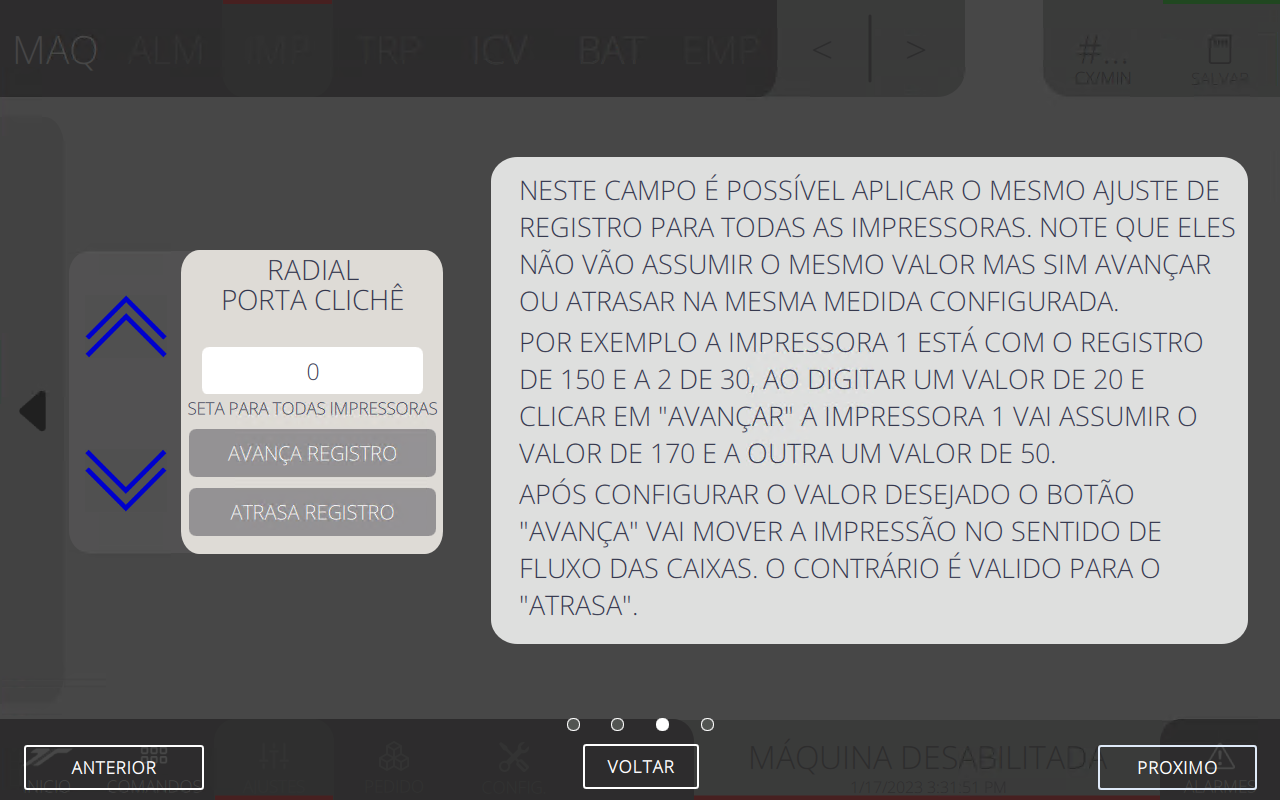
\includegraphics[width=576 px,height=360 px]{src/imagesICV/04-printters/01-printters/settings/12.png}
\end{figure}
\vspace*{\fill}

\newpage
\thispagestyle{fancy}
\vspace*{40 pt}
\subsection{Pressão rolo anilox}
\vspace*{\fill}
\begin{figure}[h]
    \centering
    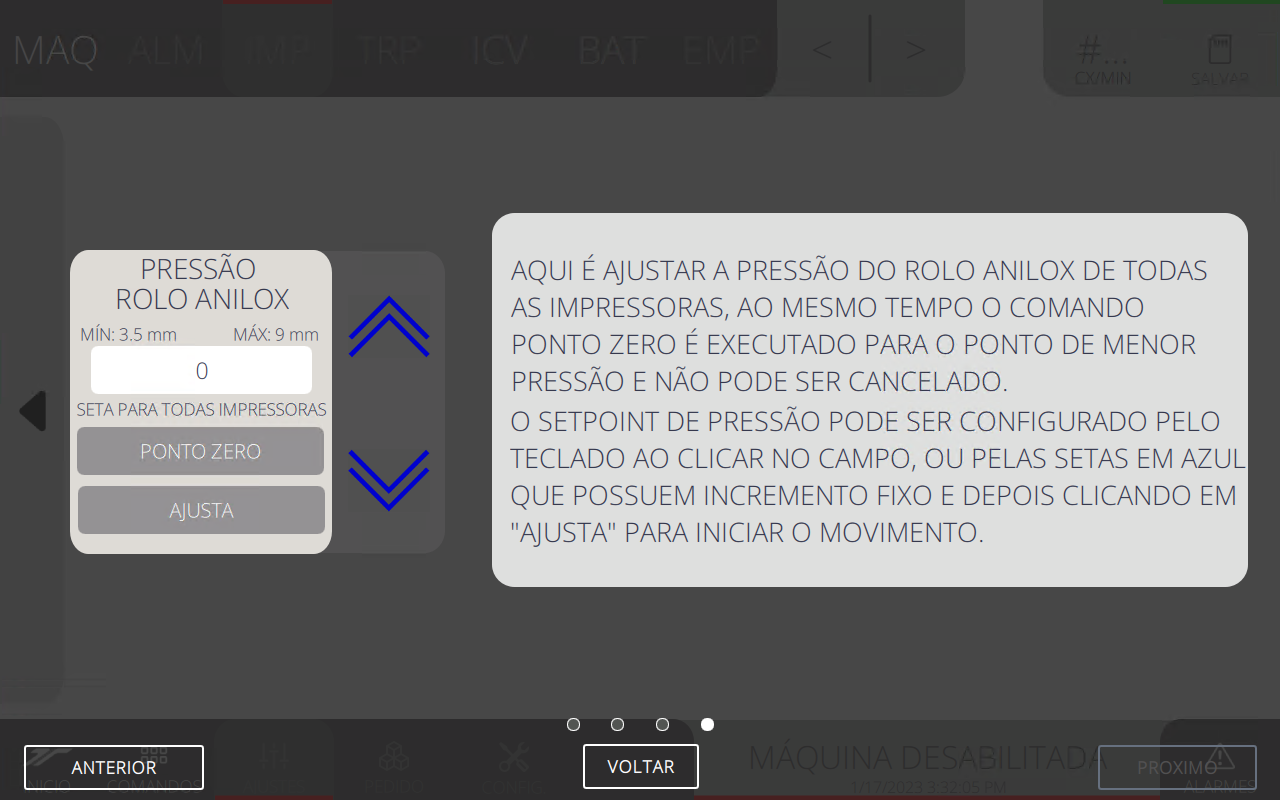
\includegraphics[width=576 px,height=360 px]{src/imagesICV/04-printters/01-printters/settings/13.png}
\end{figure}
\vspace*{\fill}